\documentclass[conference]{IEEEtran}
\IEEEoverridecommandlockouts

\usepackage{cite}
\usepackage{amsmath,amssymb,amsfonts}
\usepackage{graphicx}
\usepackage{textcomp}
\usepackage{xcolor}
\usepackage{hyperref}
\usepackage{enumitem}
\usepackage{pdfpages}
\usepackage{booktabs}
\usepackage{lipsum}

\hypersetup{
    colorlinks=true,
    linkcolor=black,
    urlcolor=black,
    citecolor=black,
}

\begin{document}
    \title{Towards multi-modal traffic prediction: a car and wheelchair case study}
    \author{
        \IEEEauthorblockN{Pierre LAPOLLA}
        \IEEEauthorblockA{
            \textit{LyRIDS ECE-Paris}\\
            Paris, France \\
            pierre.lapolla@edu.ece.fr
        }
        \and
        \IEEEauthorblockN{Guilherme MEDEIROS MACHADO}
        \IEEEauthorblockA{
            \textit{LyRIDS ECE-Paris}\\
            Paris, France \\
            gmedeirosmachado@ece.fr
        }
        \and
        \IEEEauthorblockN{Frédéric RAVAUT}
        \IEEEauthorblockA{
            \textit{LyRIDS ECE-Paris}\\
            Paris, France \\
            frederic.ravaut@ece.fr
        }
    }
    \maketitle

    \begin{abstract}
        Itinerary recommendation systems are used on a daily basis by a wide range of people, to go from a starting
        place to their destination.
        However, most existing systems do not consider accessibility constraints specific to wheelchair users.
        There is also not much data available on wheelchair users itinerary.
        In this context, this paper proposes an adaptation and evaluation of an existing itinerary recommendation
        system: Diffusion Convolutional Recurrent Neural Network (DCRNN)~\cite{DCRNN}.
        This adaptation is capable to handle multiple locomotion modes, specifically cars and wheelchairs, and computes
        the time required to travel from point A to point B\@.
        Besides the model adaptation, this study proposes a method to derive wheelchair traffic data from a dataset of
        car traffic data.
        Finally, the evaluation of the model is performed through the comparison to a baseline using the Mean Absolute
        Error (MAE) and Mean Squared Error (MSE) error metrics.
        The source code is available at \url{https://github.com/Deldrel/stage_ing4}.
    \end{abstract}

    \begin{IEEEkeywords}
        graph neural network, traffic prediction, wheelchair
    \end{IEEEkeywords}


    \section{Introduction}\label{sec:introduction}
    The need for itinerary recommendation systems has been significantly met by large platforms like Google Maps, Waze, and
Apple Maps.
They offer a wide range of functionalities, including itineraries for mobility-impaired users.
However, if a user needs to get around using a wheelchair, the options are much more limited.
For instance, any of the broadly known itinerary recommendation systems are capable of computing the time to go
somewhere by using solely the wheelchair as transportation mode.
Additionally, these companies collect private data, raising concerns about user privacy.
To address these issues, there is a growing need for an open-source model that can provide comprehensive itinerary
recommendations for all modes of transportation, including car, bike, wheelchair and walking.
\vspace{1em}

A graph is defined as follows: $G = (V, E)$, where $V$ is the set of nodes and $E$ is the set of edges.
Graphs allows complex representations of data outside Euclidean space.
Common Convolutional Neural Networks (CNNs) assume that the data is in a grid-like structure, this works well for images
but not for our case.
As traffic occurs on a road network that can be represented as a graph, we need a Graph Neural Network (GNN).
These type of neural networks allow us to perform complex operations on graph structures.
These operations enable the capture of spatial and temporal dependencies in the data, which is crucial for a problem
like traffic prediction.
\vspace{1em}

Multi-modal traffic prediction faces multiple challenges.
The first one is about data sources, as data collection on multiple modes of transportation within the same area has
never been done before.
The artificial intelligence model is the second challenge.
Managing various locomotion modes and capturing the temporal and spatial dependencies of traffic is a challenging task.
Finally, the third challenge is about scalability.
Scalability is needed for accurate real-time traffic prediction.
\vspace{1em}

To demonstrate the feasibility of multi-modal traffic prediction, we propose a model that can take in consideration cars
and wheelchairs as transportation modes.
Wheelchair users often faces unique challenges in mobility, such as inaccessible roads or sidewalks.
Given such challenges there is a need for a model that is capable of providing predictions for multiple kinds of
transportation including the wheelchairs.
\vspace{1em}

This paper proposes an adaptation of the Diffusion Convolutional Recurrent Neural Network (DCRNN) model~\cite{DCRNN}
to handle the complexity of multi-modal traffic prediction.
The DCRNN model take temporal sequences of traffic data from the METR-LA dataset~(\ref{subsec:derivation}
) and predicts the next sequence.
Our approach includes:
\begin{itemize}
    \item \textbf{Model Adaptation}:
    Enhancing the DCRNN model to take into account specifically cars and wheelchairs.
    \item \textbf{Data Derivation}:
    Developing a method to derive wheelchair traffic data from car traffic data in the METR-LA dataset.
\end{itemize}
\vspace{1em}



    \section{Related Work}\label{sec:related-work}
    Graph Neural Networks (GNNs) are often used traffic prediction tasks, due to their ability to model complex
spatial-temporal data.
The groundwork~\cite{DCRNN}
introduces a combination of diffusion convolution and gated recurrent units to capture both spatial and temporal
dependencies of traffic data.
Other studies show the potential of GNNs in complex tasks,~\cite{Wu2019A}
introduces categories of GNNs and surveys their applications.
Multi-modal traffic prediction is achieved by combining data from multiple sources like cars or bikes.
\cite{zhang2017deep} uses a deep spatio-temporal residual network to predict crowd flows.
They use data from taxis and bikes, proving the usefulness of multi-modal data to enhance performances.
Accessibility for mobility-impaired people is a growing area of research.
\cite{repetto2022developing} developed an accessibility index to evaluate public transports.
They emphasize the importance of integrating accessibility to our systems.
\vspace{1em}



    \section{Experiments}\label{sec:experiments}
    \subsection{Model Adaptation}\label{subsec:model-adaptation}
Our approach adapts DCRNN model~\cite{DCRNN} to take in consideration the wheelchair traffic.
This model captures the spatial dependency of traffic data using a custom diffusion convolution operation.
The temporal dependency is captured using Gated Recurrent Units (GRU) where matrix multiplications are replaced by
the diffusion convolution operation to create a Diffusion Convolution Gated Recurrent Unit (DCGRU).
We kept the encoder-decoder architecture of the DCRNN, but we modified some of the layers.
The model's architecture is shown in Fig.~\ref{fig:model}.
Such modifications are:

\begin{itemize}
    \item \textbf{DCGRU Cell}:
    The diffusion convolution operation in the DCGRU cell is replaced by a custom convolution that inherits from the
    MessagePassing class of the PyTorch Geometric library.
    \item \textbf{Attention Mechanism}:
    An attention mechanism is added to the model to allow the capture of different locomotion modes tendencies.
\end{itemize}
\vspace{1em}

The MessagePassing class is the base of building graph neural networks layers in PyTorch Geometric.
It allows our model to capture the spatial dependency of the graph traffic data.
It works by applying a function on features of neighboring nodes and aggregating the results, we use the addition as the
aggregation function.
It then combines the node features with the aggregated results using a fully connected layer to update the node
representation.
Attention mechanisms add trainable parameters that act like importance weights to the model.
Our model uses a multi-headed attention mechanism that allows it to differentiate between cars and wheelchairs.
\vspace{1em}

\begin{figure*}[htbp]
    \centering
    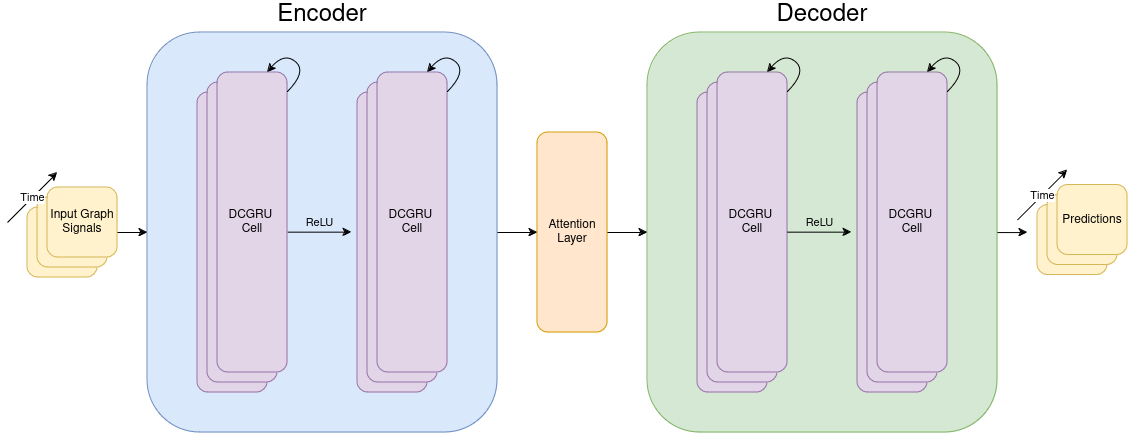
\includegraphics[width=1\textwidth]{images/model}
    \caption{
        Adapted DCRNN Model Architecture.
    }
    \label{fig:model}
\end{figure*}

\subsection{Derivation}\label{subsec:derivation}
Due to a massive lack of wheelchair traffic in the literature, this paper proposes a method to derive wheelchair data
from car traffic data.
METRopolitan Los Angeles (METR-LA) contains data about traffic information collected from loop detectors in the highway
of Los Angeles.
This dataset contains data about vehicle speed in miles per hour from 207 sensors, collected between March 1st, 2012 and
June 30th, 2012 that is aggregated into 5 minutes windows and normalized using Z-Score normalization.
From the data a graph is build using a weighted adjacency matrix $W$
where the weights represent the distance between the sensors, this matrix is build using a thresholded Gaussian kernel
weighting function~\cite{Shuman_2013}~\eqref{eq:tresholded_gaussian_kernel}.
Where $\text{dist}(i,j)$ is the distance between sensor $i$ and sensor $j$, $\sigma$
is the standard deviation of the distances and $\kappa$ is an arbitrary threshold.
\vspace{1em}

\begin{equation}
    W_{i,j} =
    \begin{cases}
        \exp\left( -\frac{\left[\text{dist}(i,j)\right]^2}{2\sigma^2} \right) & \text{if } \text{dist}(i,j) \leq \kappa
        \\
        0 & \text{otherwise}
    \end{cases}\label{eq:tresholded_gaussian_kernel}
\end{equation}
\vspace{1em}

We get accessibility data for each sensor we have using OpenStreetMap~\cite{OpenStreetMap}.
Every location in the database, either node, way or relation, can have tags that describe the location.
The tag we are interested in is the \textit{wheelchair} tag, it has 3 possible values: \textit{yes, limited, no}.
We look in a 500 meters radius around each sensor every accessibility tag and use~\eqref{eq:accessibility_score}
to compute an accessibility score for each sensor.
Where $x$ is the number of \textit{yes} tags and $y$ the number of \textit{no} tags in the circle area.
The sensor locations and search areas are shown in Fig.~\ref{fig:map}.
Equation~\eqref{eq:accessibility_score}, shown in Fig.~\ref{fig:accessibility_score_function}
,  allows areas that have more \textit{yes}
tags to have a higher score, while also rewarding areas that have more data available.

\begin{equation}
    f(x, y) = \frac{x}{x + y} \times \log(x + y + 1)\label{eq:accessibility_score}
\end{equation}
\vspace{1em}

\begin{figure}[htbp]
    \centering
    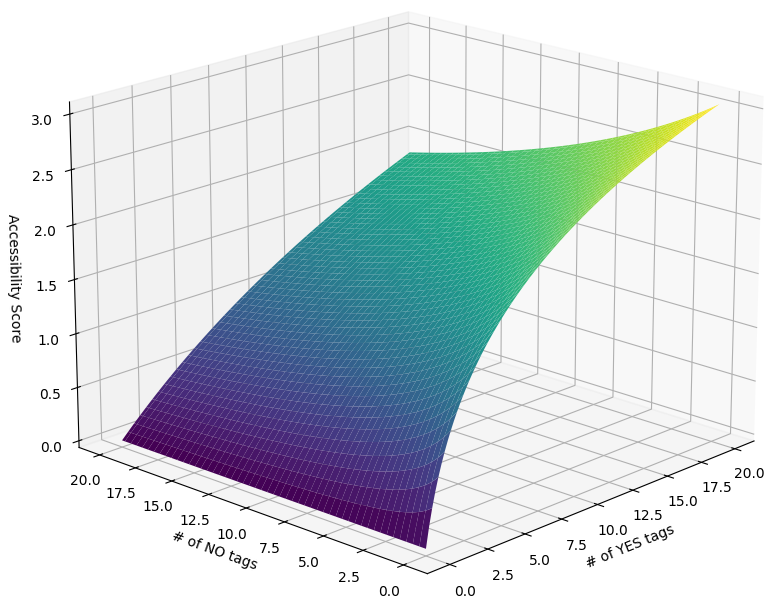
\includegraphics[width=0.5\textwidth]{images/accessibility_score_function}
    \caption{Accessibility score distribution of~\eqref{eq:accessibility_score}.}
    \label{fig:accessibility_score_function}
\end{figure}

\begin{figure}[htbp]
    \centering
    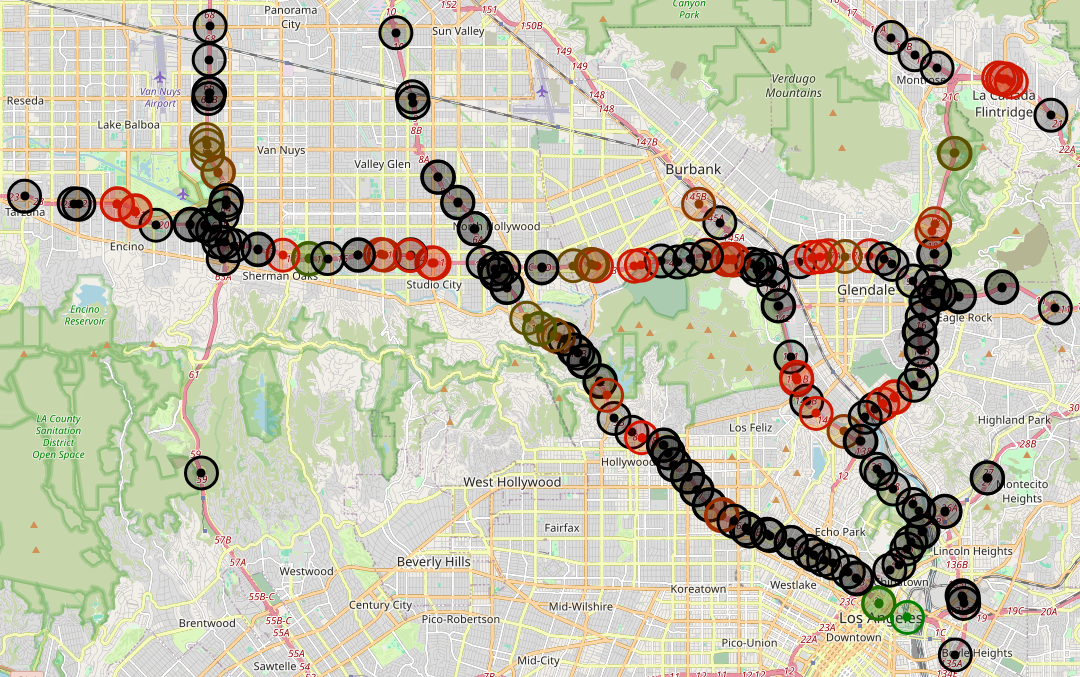
\includegraphics[width=0.5\textwidth]{images/map}
    \caption{
        Map of the sensors with their accessibility score and 500 meters radius around them.
        The sensors are colored based on their score, red being the lowest and green the highest.
        Every black sensor indicates that there is no accessibility data available.
    }
    \label{fig:map}
\end{figure}

We apply a linear transformation to the original traffic speed data to get wheelchair speeds between 0 and 4, where 4 is
a value from~\cite{FreedomMobility}.
We add some noise to the data to slightly change the values and make the model more robust.
We finally multiply our values by the accessibility score and apply a min/max scaling to end with values between 0 and
4.

\subsection{Training}\label{subsec:training}
The implementation uses PyTorch, PyTorch Geometric, PyTorch Lightning and WandB for monitoring.
We split the data into a training (70\%), validation (10\%) and test (20\%) sets.
The inputs are shaped as follows: (number of samples, number of sensors, sequence length, number of features) e.g. (
29977, 207, 12, 4).
We do not normalize the speed feature.
The sequence length is 12, which corresponds to 1 hour of data and the features are:

\begin{itemize}
    \item speed (in miles per hour)
    \item hour of the day
    \item day of the week
    \item locomotion mode (hot encoded)
\end{itemize}
\vspace{1em}

The model is evaluated using three metrics:
\begin{itemize}
    \item Mean Absolute Error (MAE)~\eqref{eq:mae}
    \item Root Mean Squared Error (RMSE)~\eqref{eq:rmse}
\end{itemize}
Where $y$ is the ground truth, $\hat{y}$ the prediction and $n$ the batch size.

\begin{equation}
    MAE(y, \hat{y}) = \frac{1}{n} \sum_{i=1}^{n} \left| y_i - \hat{y}_i \right|\label{eq:mae}
\end{equation}

\begin{equation}
    RMSE(y, \hat{y}) = \sqrt{\frac{1}{n} \sum_{i=1}^{n} \left( y_i - \hat{y}_i \right)^2}\label{eq:rmse}
\end{equation}
\vspace{1em}


    \section{Results}\label{sec:results}
    The model's performance was evaluated using the MAE and RMSE metrics.
Table~\ref{tab:model_performance_comparison} shows a comparison between our model and the baseline, including the DCRNN~
\cite{DCRNN} and the STGM~\cite{LABLACK2023120281}.
The horizon is set to 1 hour (12 time steps).

NOTE: further experiments are in progress to get better comparisons to the baseline, like using other metrics and other
horizons.

\begin{figure}[htbp]
    \centering
    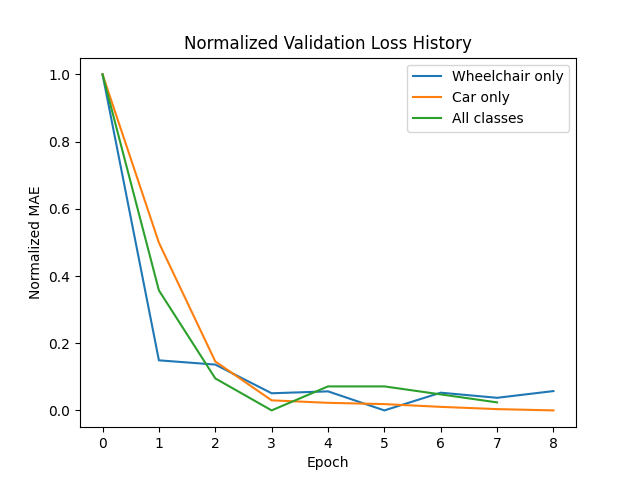
\includegraphics[width=0.5\textwidth]{images/normalized_val_losses}
    \caption{
        Plot of normalized validation losses during 3 trainings, one with only car data,
        one with only wheelchair data and one with both.
    }
    \label{fig:normalized_val_losses}
\end{figure}

\begin{table}[htbp]
    \caption{Model performance comparison on the METR-LA dataset, with~\cite{DCRNN},
        ~\cite{LABLACK2023120281}}
    \center
    \begin{tabular}{@{}llllll@{}}
        \toprule
        \textbf{Metric} & \textbf{STGM} & \textbf{DCRNN} & \multicolumn{3}{c}{\textbf{Adapted DCRNN}} \\
        & \textbf{Cars} & \textbf{Cars} & \textbf{Cars} & \textbf{Wheelchairs} & \textbf{All} \\
        \midrule
        MAE  & 3.60          & 3.23          & 2.67          & 0.08                 & 6.84         \\
        RMSE & 7.59          & 7.09          & 8.59          & 0.18                 & 14.8         \\
        \bottomrule
    \end{tabular}
    \label{tab:model_performance_comparison}
\end{table}


    \section{Discussion}\label{sec:discussion}
    The results of our adapted model are promising but also reveal areas that require further research.
\begin{itemize}
    \item \textbf{Car Traffic Prediction}:
    Our model achieve a similar performance than the DCRNN baseline in terms of MAE and RMSE\@.
    This suggests that our modifications are not penalizing the model's ability to handle car traffic data.
    \item \textbf{Wheelchair Traffic Prediction}:
    There is no baseline for wheelchair traffic prediction, as this is a novel contribution of our study.
    The results are promising and suggest that the model can effectively handle wheelchair data.
    The losses are very low compared to the car traffic prediction, this indicates better accuracy but needs to be
    contextualized.
    As our speed feature is not normalized and wheelchair speeds are significantly lower than car speeds, losses are
    expected to be lower.
    \item \textbf{Multi-Modal Traffic Prediction}:
    The model's performance on multi-modal traffic prediction, combining cars and wheelchair data, is not as good as
    expected.
    This confirms the complexity of handling multiple locomotion modes with a single model.
    The increase of the MAE and RMSE could come from the data and/or the model architecture.
\end{itemize}
\vspace{1em}

Our study introduces some implications and limitations, a first implication is data derivation.
Although it offers a new methodology, the process of obtaining wheelchair traffic data from car traffic data may add
many biases.
Even if this method is innovative, it highlights the need for dedicated data collection on other locomotion modes than
cars.
The second implication is scalability, as the performance on the METR-LA dataset suggests potential scalability.
But the differences in results between cars, wheelchairs and both indicate otherwise.
Lastly, the model generalization is a limitation.
While the model performs well on the METR-LA dataset, its generalization to other areas remains untested.
Further efforts are needed to evaluate the model across varied datasets.
\vspace{1em}

We propose several directions for future work.
\begin{itemize}
    \item \textbf{Data Collection}:
    Conducting new data collection efforts could be beneficial for the research community.
    Data from other countries or cities could allow more tests for better models.
    \item \textbf{Model Improvement}:
    Further improvements to the model architecture could enhance its performance on multi-modal traffic prediction.
    Adding other techniques or dividing the prediction task between multiple models are possible directions of research.
    \item \textbf{Adding Accessibility Features}:
    Adding more accessibility features to the data, such as public transport accessibility, could emphasize the social
    contribution of our study.
    \item \textbf{Model Comparison}:
    We could improve our understanding of the model's performance by comparing it to other models, and measuring its
    performance on different metrics and horizons.
\end{itemize}
\vspace{1em}



    \section{Conclusion}\label{sec:conclusion}
    Our article introduced a new method for multi-modal traffic prediction that takes into account both car and wheelchair
traffic by modifying the DCRNN model.
We used the METR-LA dataset to derive wheelchair traffic data from car traffic data, solving the lack of wheelchair
traffic data.
With the added attention mechanism and modified convolution operation, our model performed as intended on car and
wheelchair data independently.
However, the model's performance on multi-modal traffic prediction was not as good as expected, with MAE loss of 6.84
and RMSE loss of 14.8.
This behavior could come from our methodology, either from the model architecture or the data derivation.
This study establishes new ideas for research around inclusivity in traffic prediction.
In order to contribute to the research community, we offer recommendations for future work like accessibility data
collection and model improvements.
\vspace{1em}

    \section*{Acknowledgment}
    The authors would like to thank Thomas ROUSTAN and all other colleagues for their valuable assistance and support
    during this project.
    \vspace{1em}

    \bibliographystyle{unsrt}
    \bibliography{../out/references}

\end{document}
